% 1. Стиль и язык
\documentclass[utf8x, 14pt]{G7-32} % Стиль (по умолчанию будет 14pt)
% Остальные стандартные настройки убраны в preamble.inc.tex.
\sloppy

% Настройки стиля ГОСТ 7-32
% Для начала определяем, хотим мы или нет, чтобы рисунки и таблицы нумеровались в пределах раздела, или нам нужна сквозная нумерация.
\EqInChapter % формулы будут нумероваться в пределах раздела
\TableInChapter % таблицы будут нумероваться в пределах раздела
\PicInChapter % рисунки будут нумероваться в пределах раздела

% Добавляем гипертекстовое оглавление в PDF
\usepackage[
bookmarks=true, colorlinks=true, unicode=true,
urlcolor=black,linkcolor=black, anchorcolor=black,
citecolor=black, menucolor=black, filecolor=black,
]{hyperref}

\AfterHyperrefFix

\usepackage{microtype}% полезный пакет для микротипографии, увы под xelatex мало чего умеет, но под pdflatex хорошо улучшает читаемость

% Тире могут быть невидимы в Adobe Reader
\ifInvisibleDashes
\MakeDashesBold
\fi

\usepackage{graphicx}   % Пакет для включения рисунков

% С такими оно полями оно работает по-умолчанию:
% \RequirePackage[left=20mm,right=10mm,top=20mm,bottom=20mm,headsep=0pt,includefoot]{geometry}
% Если вас тошнит от поля в 10мм --- увеличивайте до 20-ти, ну и про переплёт не забывайте:
\geometry{right=20mm}
\geometry{left=30mm}
\geometry{bottom=20mm}
\geometry{ignorefoot}% считать от нижней границы текста


% Пакет Tikz
\usepackage{tikz}
\usetikzlibrary{arrows,positioning,shadows}

% Произвольная нумерация списков.
\usepackage{enumerate}

% ячейки в несколько строчек
\usepackage{multirow}

% itemize внутри tabular
\usepackage{paralist,array}

%\setlength{\parskip}{1ex plus0.5ex minus0.5ex} % разрыв между абзацами
\setlength{\parskip}{1ex} % разрыв между абзацами
\usepackage{blindtext}

% Центрирование подписей к плавающим окружениям
%\usepackage[justification=centering]{caption}
\usepackage{newfloat}

% Алгоритмы
\usepackage[ruled,vlined]{algorithm2e}
\SetAlgorithmName{Алгоритм}{алгоритм}{Список алгоритмов}

% Математика
\usepackage{amsmath}

% Код
\usepackage{courier}
\usepackage{listings}             % Include the listings-package

% Изображения
% \usepackage[demo]{graphicx}
% \usepackage{caption}
\usepackage{subcaption}
\graphicspath{ {Pictures/} }

\DeclareFloatingEnvironment[
placement={!ht},
name=Equation
]{eqndescNoIndent}
\edef\fixEqndesc{\noexpand\setlength{\noexpand\parindent}{\the\parindent}\noexpand\setlength{\noexpand\parskip}{\the\parskip}}
\newenvironment{eqndesc}[1][!ht]{%
    \begin{eqndescNoIndent}[#1]%
\fixEqndesc%
}
{\end{eqndescNoIndent}}
\setcounter{page}{5}
\setmainfont{Times New Roman}
\setlength{\parskip}{0em}
% Настройки листингов.
% \ifPDFTeX
% 8 Листинги

\usepackage{listings}

% Значения по умолчанию
\lstset{
  keepspaces=true,
  basicstyle= \footnotesize\ttfamily,
  breakatwhitespace=true,% разрыв строк только на whitespacce
  breaklines=true,       % переносить длинные строки
%   captionpos=b,          % подписи снизу -- вроде не надо
  inputencoding=koi8-r,
  numbers=left,          % нумерация слева
  numberstyle=\footnotesize,
  showspaces=false,      % показывать пробелы подчеркиваниями -- идиотизм 70-х годов
  showstringspaces=false,
  showtabs=false,        % и табы тоже
  stepnumber=1,
  tabsize=4,              % кому нужны табы по 8 символов?
  frame=single
}

% Стиль для псевдокода: строчки обычно короткие, поэтому размер шрифта побольше
\lstdefinestyle{pseudocode}{
  basicstyle=\small,
  keywordstyle=\color{black}\bfseries\underbar,
  language=Pseudocode,
  numberstyle=\footnotesize,
  commentstyle=\footnotesize\it
}

% Стиль для обычного кода: маленький шрифт
\lstdefinestyle{realcode}{
  basicstyle=\scriptsize,
  numberstyle=\footnotesize
}

% Стиль для коротких кусков обычного кода: средний шрифт
\lstdefinestyle{simplecode}{
  basicstyle=\footnotesize,
  numberstyle=\footnotesize
}

% Стиль для BNF
\lstdefinestyle{grammar}{
  basicstyle=\footnotesize,
  numberstyle=\footnotesize,
  stringstyle=\bfseries\ttfamily,
  language=BNF
}

% Определим свой язык для написания псевдокодов на основе Python
\lstdefinelanguage[]{Pseudocode}[]{Python}{
  morekeywords={each,empty,wait,do},% ключевые слова добавлять сюда
  morecomment=[s]{\{}{\}},% комменты {а-ля Pascal} смотрятся нагляднее
  literate=% а сюда добавлять операторы, которые хотите отображать как мат. символы
    {->}{\ensuremath{$\rightarrow$}~}2%
    {<-}{\ensuremath{$\leftarrow$}~}2%
    {:=}{\ensuremath{$\leftarrow$}~}2%
    {<--}{\ensuremath{$\Longleftarrow$}~}2%
}[keywords,comments]

% Свой язык для задания грамматик в BNF
\lstdefinelanguage[]{BNF}[]{}{
  morekeywords={},
  morecomment=[s]{@}{@},
  morestring=[b]",%
  literate=%
    {->}{\ensuremath{$\rightarrow$}~}2%
    {*}{\ensuremath{$^*$}~}2%
    {+}{\ensuremath{$^+$}~}2%
    {|}{\ensuremath{$|$}~}2%
}[keywords,comments,strings]

% Подписи к листингам на русском языке.
\renewcommand\lstlistingname{Листинг}
\renewcommand\lstlistlistingname{Листинги}

% \else
% \usepackage{local-minted}
% \fi

% Полезные макросы листингов.
% Любимые команды
\newcommand{\Code}[1]{\textbf{#1}}


\begin{document}

\frontmatter % выключает нумерацию ВСЕГО; здесь начинаются ненумерованные главы: реферат, введение, глоссарий, сокращения и прочее.


%\listoffigures                         % Список рисунков

%\listoftables                          % Список таблиц

%\NormRefs % Нормативные ссылки 
% Команды \breakingbeforechapters и \nonbreakingbeforechapters
% управляют разрывом страницы перед главами.
% По-умолчанию страница разрывается.

% \nobreakingbeforechapters
% \breakingbeforechapters

\tableofcontents

% \printnomenclature % Автоматический список сокращений

\Introduction
Стеганография --- это практика сокрытия сообщения внутри другого сообщения или физического объекта.
Тогда как криптография скрывает содержимое сообщение, стеганография скрывает сам факт существования какого-либо сообщения. 

Стеганография часто используется совместно с криптографией, дополняя ее.
Стеганографические методы сокрытия сообщения снижают вероятность обнаружения самой передачи сообщения.
Если сообщение к тому же зашифровано, то это обеспечивает еще большую защищенность. 

В настоящее время наибольшее распространение получила цифровая стеганография.
Особенностью цифровой стеганографии является сокрытие информации внутри других цифровых объектов,
таких как текст, изображения, видео, аудио и другие.
Со все большим возрастанием роли интернет-технологий в жизни человека значимость стеганографии также возрастает.

Области применения стеганографии включают в себя:
\begin{enumerate}
    \item Защита авторского права и DRM (digital rights management).
    \item Незаметная передача информации.
    \item Защита конфиденциальной информации от несанкционированного доступа.
\end{enumerate}

Цифровая стеганография является молодым и бурно развивающимся направлением.
Несмотря на свою востребованность, стеганография очень слабо освещается в программах обучения информационной безопасности.
Моя работа призвана восполнить этот пробел.

В своей работе я хочу рассмотреть основные стеганографические алгоритмы, определить области их применения,
достоинства и недостатки, а также провести анализ возможных уязвимостей этих алгоритмов.


\mainmatter % это включает нумерацию глав и секций в документе ниже

\chapter{Теоретические аспекты изучаемой темы}

\section{Основные понятия}

\begin{enumerate}
    \item Стеганографическая система (стегосистема) --- совокупность методов и средств,
    используемых для создания скрытого канала для передачи информации.
    Основные требования, предъявляемые к стегосистеме:
    \begin{enumerate}
        \item Безопасность системы определяется секретностью ключа.
        Это означает, что даже если потенциальный враг представляет работу стеганографической системы
        и статистические характеристики сообщений и контейнеров,
        это не дает ему дополнительных преимуществ при выявлении
        наличия или отсутствия сообщения в конкретном контейнере.
        \item При обнаружении противником наличия скрытого сообщения
        он не должен смочь извлечь сообщение до тех пор, пока он не будет владеть ключом.
        \item Алгоритм сокрытия информации не нарушает ее целостность и аутентичность.
        В некоторых случаях дополнительно требуется,
        чтобы алгоритм обеспечивал целостность сообщения при деформации контейнера.
        \item Система с цифровым водяным знаком должна иметь низкую вероятность ложного обнаружения скрытого сообщения.
    \end{enumerate}
    \item Сообщение --- информация, передачу которой нужно скрыть.
    \item Контейнер --- любая информация,
    используемая для сокрытия тайного сообщения. Контейнер может находиться в одном из двух состояний:
    \begin{enumerate}
        \item Пустой контейнер --- контейнер, не содержащий сообщение.
        \item Заполненный контейнер (стегоконтейнер) --- контейнер, содержащий сообщение.
    \end{enumerate}
    \item Стеганографический канал (стегоканал) --- канал передачи стегоконтейнера.
    \item Ключ (стегоключ) --- секретный ключ, нужный для сокрытия стегоконтейнера.
    По аналогии с криптографией стегоключи подразделяются на 2 типа:
    \begin{enumerate}
        \item Закрытый стегоключ.
        В системах с закрытым стегоключем ключ должен быть создан до начала обмена сообщениями,
        либо передан по защищенному каналу связи.
        \item Открытый стегоключ. Такой ключ может быть передан по открытому незащищенному каналу связи.
        Открытый стегоключ должен обладать таким свойством, чтобы по нему вычислительно нецелесообразно
        было восстанавливать закрытый ключ.
    \end{enumerate}
\end{enumerate}

\section{Цифровые водяные знаки и цифровые отпечатки}

Цифровой водяной знак (ЦВЗ) --- технология, созданная для защиты авторский прав на цифровые объекты.
В связи с быстрым развитием информационных технологий все более актуальным становится
вопрос защиты авторских прав и интеллектуальной собственности, представленной в цифровом виде.
Примерами цифровых объектов могут выступать аудиозаписи, видеозаписи, изображения, электронные книги и другие. 
ЦВЗ могут быть как видимыми, так и невидимыми. Решение о наличии в цифровом объекте невидимого ЦВЗ принимаются
на основе процедуры декодирования.

В общем виде стегосистема ЦВЗ может быть разбита на части следующим образом:
\begin{enumerate}
    \item Прекодер --- часть, которая приводит ЦВЗ к удобному для встраивания в стегоконтейнер виду.
    \item Стегокодер --- часть, которая вкладывает сообщение в стегоконтейнер.
    \item Выделение встроенного сообщения --- процедура, выделяющие сообщение из стегоконтейнера.
    \item Стегодетектор --- часть, определяющая наличие ЦВЗ.
    \item Декодер --- часть, восстанавливающая исходное сообщение.
\end{enumerate}

Контейнер, содержащий ЦВЗ, может подвергаться преднамеренным атакам или случайным помехам.
Стегосистема ЦВЗ должна обеспечивать как различимость самого стегоконтейнера человеком,
потому как в качестве стегоконтейнера выступает интеллектуальная собственность,
нацеленная на конечного потребителя, так и различимость ЦВЗ стегодетектором,
который может подтвердить или опровергнуть авторские права на интеллектуальную собственность.
В связи с этим в стегосистемах ЦВЗ применяется помехоустойчивое кодирование и метод широкополосного сигнала.

Одной из основных характеристик ЦВЗ является надежность.
Под надежность понимается устойчивость к различным деформациям контейнера.
По отношению к этой характеристика ЦВЗ распадается на три класса:
\begin{enumerate}
    \item Хрупкие.
    Такие ЦВЗ разрушается при небольших модификациях заполненного стегоконтейнера.
    Такие ЦВЗ применяются для аутентификации сигнала.
    Например, такие ЦВЗ используются для подтверждения подлинности цифрового объекта.
    \item Полухрупкие.
    Такие ЦВЗ чувствительны к некоторым преобразованиям контейнера и нечувствительны к другим.
    Например, ЦВЗ, встроенное в изображение, может быть нечувствительно к его компрессии,
    но в то же время быть чувствительно к вырезке из этого изображения фрагмента.
    \item Робастные или надежные.
    Такие ЦВЗ устойчивы к разным видам воздействия на контейнер.
    Такие ЦВЗ часто применяются при защите от копирования.
\end{enumerate}

Похожим на ЦВЗ, но отличающимся понятием является цифровой отпечаток.
ЦВЗ предполагает встраивание одного и того же сообщения в различные контейнеры.
В случае же цифрового отпечатка в каждый контейнер встраивается уникальное сообщение.
Часто областью применения цифровых отпечатков становится защита исключительного права.
В качестве сообщения в таком случае встраивается информация, указывающая на идентифицирующие данные покупателя.
Эти данные позволят отследить источник распространения, если произойдет утечка стегоконтейнера.

\section{Обобщенные стеганографические методы}
К настоящему моменту разработано множество стеганографических методов скрытия информации.
Для их систематичного изучения удобно группировать их по схожим признакам.
\begin{enumerate}
    \item Пространственные методы. Особенностью этих методов является сокрытие информации напрямую
    в пространственной области контейнера. Например,
    в случае звукового контейнера  таким пространством могут быть семплы,
    а в случае изображения --- пиксели.
    \item Частотные методы. Такие методы сначала используют одно из интегральный преобразований сигнала,
    чтобы перейти в его частотную область. Далее кодирование сообщение производится за счет изменения частотных
    характеристик сигнала. После этого используется обратное преобразование, чтобы получить модифицированный сигнал,
    содержащий закодированное сообщение.
    \item Алгоритмы, использующие особенности формата файла. Такие алгоритмы как правило записывают
    сообщение в метаданные файла или в иные неиспользуемые поля файла.
\end{enumerate}

\section{Стегоанализ}
Стегоанализ --- это наука о выявлении сообщений, скрытых методами стеганографии.
Задача стегоанализа --- выявить подозрительные контейнеры, определить, есть ли в них скрытое сообщение,
и, если возможно, восстановить это сообщение.

Если в случае криптоанализа аналитик начинает работу сразу с зашифрованным сообщением,
то в случае стегоанализа аналитик начинает работу с множества подозрительных файлов,
о которых как правило мало что известно. Деятельность аналитика в таком случае
начинается с сокращения этого множества файлов до подмножества, в котором файлы
скорее всего были заполнены сообщением.

Основной техникой, используемой в стегоанализе, является статистический анализ.
Сначала множество незаполненных контейнеров одного типа анализируется для получения
различной статистики. Затем эта статистка используется при классификации контейнера
как заполненного или пустого. При такой классификации могут быть использованы
самые различные наблюдения:
\begin{enumerate}
    \item Сокрытие информации может приводить к изменению статистической структуры
    контейнера, в результате чего соседние элементы контейнера становятся попарно ближе
    друг к другу. На этом основана атака хи-квадрат.
    \item Сокрытие информации увеличивает энтропию контейнера. В результате чего он
    хуже поддается сжатию. На этом основана атака с помощью алгоритмов сжатия.
\end{enumerate}
Так же для такой классификации могут быть использованы методы машинного обучения.
\chapter{Методы стеганографии}
\section{LSB}
LSB (least significant bit) --- стеганографический метод сокрытия информации, основанный на замене поседних значащих бит
элементов контейнера битами сообщения. Этот метод использует тот факт,
что уровень детализации во многих контейнерах гораздо выше того,
что может воспринять и различить человек. Следовательно,
заполенный контейнер будет неотличим от оригинального
для человеческого восприятия.

LSB обладает следующими достоинствами:
\begin{enumerate}
    \item Простота реализации.
    \item Низкая вычислительная сложность.
    \item Пустой и заполненный контейнер неразличимы для органов восприятия человека
\end{enumerate}
И недостатками:
\begin{enumerate}
    \item Метод применим лишь к контейнерам, которые хранят данные без сжатия или используют
    сжатие без потерь, так как информации, закодированная в наименее значимых битах, может
    быть потеряна в процессе сжатия.
    \item Небольшие трансформации контейнера приводят к невозможности восстановить сообщение.
    Например, если сообщение скрыто в изображении методом LSB, то небольшие линейные трансформации
    (вращение, движение, отражение, гомотетия, сжатие, растяжение) уничтожат сообщение.
\end{enumerate}

Перейдем к конкретным реализациям этого метода. Алгоритм~\ref{alg:lsb_encode}
демонстрирует псевдокод сокрытия методом LSB.
\begin{algorithm}[ht!]
    \KwData{Контейнер, Сообщение}
    \KwResult{Заполненный стегоконтейнер}
     $N \leftarrow$ Длина сообщения в битах\;
     $Message \leftarrow$ Бинарное представление сообщения\;
     $Container \leftarrow$ Массив с элементами контейнера\;
     \For{$i = 1, 2, \ldots, N$}{
         \eIf{$Container[i] \equiv Message[i] \pmod{2}$}{
             \textbf{continue\;}
         }{
             $Container[i] \leftarrow (Container[i] \land \neg 1) \lor Message[i]$\;
         }
     }
     \caption{LSB Кодирование}
    \label{alg:lsb_encode}
\end{algorithm}
Как видно, сначала сообщение преобразуется в бинарный вид,
а затем кодируется в элементах контейнера за счет изменения четности младшего бита.
Логические операции в данном случае соответствуют бинарным операциям на компьютере.
В итоге последние биты элементов контейнера в точности повторяют сообщение.
Так же можно заметить, что единственная часть алгоритма, зависящая от контейнера
--- это выделение массива элементов из контейнера. Алгоритм~\ref{alg:lsb_decode}
показывает, как декодировать сообщение из заполненного стегоконтейнера.
\begin{algorithm}[ht!]
    \KwData{Заполненный контейнер}
    \KwResult{Сообщение в бинарном представлении}
    $Message \leftarrow$ Пустой список\;
    $Container \leftarrow$ Массив с элементами контнейнера\;
    $N \leftarrow$ Длина $Container$\;
    \For{$i = 1, 2, \ldots, N$}{
        \eIf{$Container[i] \equiv 0 \pmod{2}$}{
            $Message.append(0)$\;
        }{
            $Message.append(1)$\;
        }
    }
    \caption{LSB Декодирование}
    \label{alg:lsb_decode}
\end{algorithm}

Реализуем этот алгоритм в виде класса на Python. Как уже было сказано,
существенная часть алгоритма не зависит от контейнера,
поэтому целесообразно реализовать алгоритм как абстрактный класс,
от которого будут наследоваться реализации для конкретных контейнеров.
\lstinputlisting[language=Python, style=simplecode, caption=Абстрактный класс LSB, frame=single]{Code/lsb.py}

Как видно, в методах нет циклов \textbf{for}. Они скрыты за интерфейсом библиотеки numpy.
Интерфейс библиотеки numpy позволяет нам применят операции к матрицам,
из-за чего код выглядет лаконичнее. К тому же библиотека написана на языке C,
поэтому ее код работает очень быстро.

Напишем реализацию LSB для PNG. Прежде чем реализовать метод LSB для PNG-контейнера,
имеет смысл коротко изложить формат данных PNG.

В самом общем виде PNG файл представляет из себя сигнатуру,
за которой следует последовательность блоков (chunks),
как показано на рисунке~\ref{img:png_1}
\begin{figure}[ht!]
    \caption{Общий вид формата PNG}
    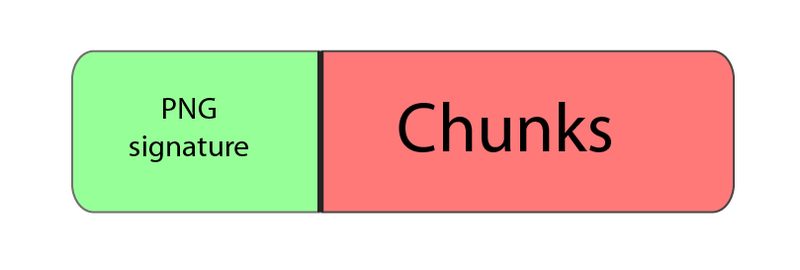
\includegraphics{PNG/1}
    \centering
    \label{img:png_1}
\end{figure}

Каждый блок состоит из четырех секций: длина, тип, содержание, CRC, --- как показано на рисунке~\ref{img:png_2}:
\begin{figure}[ht!]
    \caption{Общий вид чанка}
    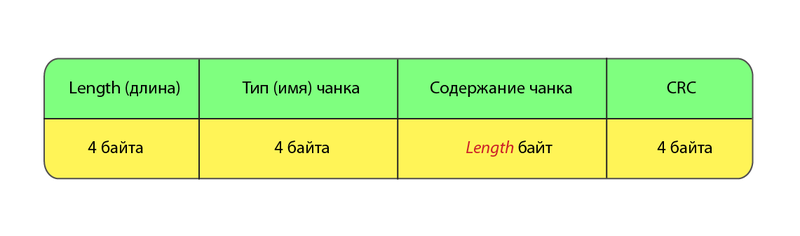
\includegraphics{PNG/2}
    \centering
    \label{img:png_2}
\end{figure}
В длине указывается длина блока в байтах. Тип указывается с помощью четырех ascii символов,
чувствительных к регистру. В следующей секции представлены данные блока.
В секции CRC записан CRC блока.

Наиболее интересными для нас являются блоки с типами IHDR и IDAT.
IHDR --- заголовочный блок, который является обязательным для PNG файла.
Он содержит следующие интересующие нас поля:
\begin{enumerate}
    \item Ширина изображения в пикселях.
    \item Высота изображения в пикселях.
    \item Битовая глубина, задающее количество бит на каждый сэмпл.
    \item Тип цвета. Возможны следующие значения:
    \begin{enumerate}
        \item Градация серого
        \item RGB
        \item Индексы из палитры
        \item Градация серого и альфа-канал
        \item RGB и альфа-канал
    \end{enumerate}
\end{enumerate}

Блок IDAT содержит сжатые данные изображения.
На данный момент поддерживается только сжатия по алгоритму deflate.

PNG изображение представимо в виде матрицы, элементами которой являются пиксели.
Чтобы закодировать сообщение в эту матрицу, склеим ее строки друг с другом,
равно как и склеим каналы, чтобы они образовали последовательность элементов.
Именно это делает метод \textbf{\_ to \_ elements}.
Такой метод одинаково хорошо подходит и для разных типов цвета: RGB, RGB и альфа-канала,
градации серого, градации серого и альфа-канала.
Чтобы из элементов получить двумерную RGB матрицу,
проделаем обратную операцию, что и далет метод \textbf{\_ from \_ elements}.

В функции \textbf{main} используем как сообщение книгу "Алиса в стране чудес" в оригинале.
Считаем файл с книгой как последовательность байт и закодируем в изображение с помощью LSB.
Далее выполним декодирование и сверим полученные данные.
Исходный код представлен в листинге~\ref{code:png}.
\lstinputlisting[language=Python, label={code:png}, style=simplecode, caption=реализация LSB для PNG, frame=single]{Code/png.py}
Сравним фотографии до заполнения сообщением методом LSB и после,
рисунок~\ref{img:lenna} и рисунок~\ref{img:lenna-lsb} соответственно.
Как видно, два рисунка визуально неотличимы,
хотя в одном из них закодировано 150 килобайт информации.
\begin{figure}[ht!]
    \caption{Оригинальное изображение}
    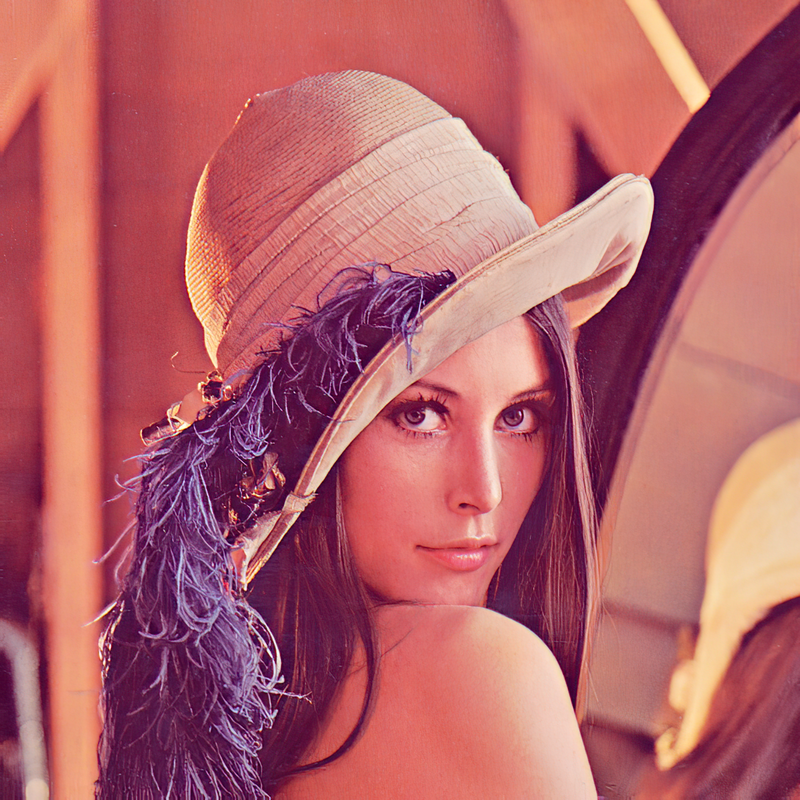
\includegraphics[width=\linewidth]{PNG/Lenna}
    \centering
    \label{img:lenna}
\end{figure}
\begin{figure}[ht!]
    \caption{Изображение после приминения LSB}
    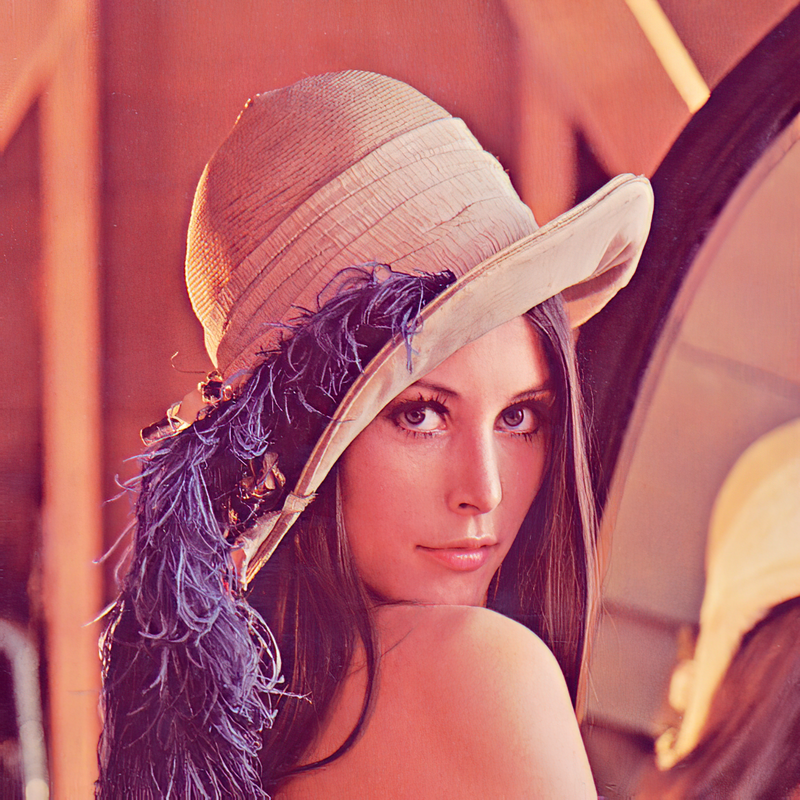
\includegraphics[width=\linewidth]{PNG/LSB_Lenna}
    \centering
    \label{img:lenna-lsb}
\end{figure}


\backmatter %% Здесь заканчивается нумерованная часть документа и начинаются ссылки

\appendix   % Тут идут приложения

\end{document}